\documentclass[titlepage, letterpaper, 12pt, oneside]{book}
% --------------------------------------------------------------------------- %
% Comment these lines out to remove the watermark
% --------------------------------------------------------------------------- %
%\usepackage[printwatermark]{xwatermark}
%\newwatermark[allpages,color=red!10,angle=90,scale=3.75,xpos=60,ypos=0]
%{DRAFT\textbullet DRAFT}

% --------------------------------------------------------------------------- %
% fontspec gives problems if you compile with pdflatex
% --------------------------------------------------------------------------- %
\usepackage{fontspec}
\setmainfont{Times New Roman}
% --------------------------------------------------------------------------- %
\usepackage[letterpaper]{geometry}
\geometry{left=1.5in, right=1.25in, top=1.25in, bottom=1.25in}
\usepackage{setspace}
\usepackage{enumitem}
\usepackage{pdfpages}
%\pagenumbering{gobble}
\usepackage{multicol}
\usepackage[section]{placeins}    % Place in a section FORCEFULLY!!
\usepackage{titlesec}             % Important for changing the titles
\usepackage{blindtext}            % Testing
\usepackage{booktabs}             % I can't remember what this is for...
\usepackage{verbatim}
\usepackage{dirtytalk}            % Use \say{thing you want in quotations}
\usepackage{csquotes}             % For block quotes
\definecolor{mtsublue}{cmyk}{1.0,0.44,0,0} % Defines an MTSU blue
\usepackage[breaklinks=true, colorlinks=false, allbordercolors=mtsublue]{hyperref}
\usepackage{url}                  % For urls
\usepackage[labelfont = bf, font = small]{caption} %Allows for use of \caption* for non-labeled captions
\usepackage{graphicx}
\graphicspath{ {images/} }   % Put your images in the images subdirectory
\usepackage{float}
\usepackage[numbers, round]{natbib}
\bibliographystyle{plainnat}
\usepackage{todonotes}
\usepackage{caption}
\captionsetup{width = 0.7\textwidth}
\usepackage{subcaption}

\usepackage{siunitx}
\usepackage{amsmath}
\usepackage{esint}
\usepackage{mathcomp}

\usepackage{listings}
\usepackage{color}
\usepackage{dirtree}

\definecolor{dkgreen}{rgb}{0,0.6,0}
\definecolor{gray}{rgb}{0.5,0.5,0.5}
\definecolor{mauve}{rgb}{0.58,0,0.82}

\lstset{frame=tb,
    language=python,
    aboveskip=3mm,
    belowskip=3mm,
    showstringspaces=false,
    columns=flexible,
    basicstyle={\small\ttfamily},
    numbers=none,
    numberstyle=\tiny\color{gray},
    keywordstyle=\color{blue},
    commentstyle=\color{dkgreen},
    stringstyle=\color{mauve},
    breaklines=true,
    breakatwhitespace=true,
    tabsize=3
}

\pagestyle{plain}
% --------------------------------------------------------------------------- %
% TIKZ STUFF
% --------------------------------------------------------------------------- %
\usepackage{tikz}
\usetikzlibrary{
    shapes,
    arrows,
    decorations.markings,
    positioning,
}

% Define block styles
% --------------------------------------------------------------------------- %
\tikzset{
    startstop/.style ={
        rectangle,
        rounded corners,
        minimum width=2cm,
        minimum height=1cm,
        text centered,
        thick,
        draw,
    },
    io/.style = {
        trapezium,
        trapezium left angle=70,
        trapezium right angle=110,
        text width=2cm,
        minimum height=1cm,
        align=center,
        thick,
        draw,
    },
    process/.style = {
        rectangle,
        text width=5cm,
        minimum height=1cm,
        align=center,
        thick,
        draw,
    },
    decision/.style = {
        diamond,
        text width=5cm,
        minimum height=1cm,
        align=center,
        thick,
        draw,
    },
}
\tikzstyle{arrow} = [
    thick,
    ->,
    >=stealth
]
% --------------------------------------------------------------------------- %

% --------------------------------------------------------------------------- %
% newcommands, newenvironments
% --------------------------------------------------------------------------- %
% Writing
% --------------------------------------------------------------------------- %
\newcommand{\comm}[1]{\textcolor{red}{[#1]}}    % inline comment command

% Math
% --------------------------------------------------------------------------- %
\newcommand{\pprime}{^{\prime}}
\newcommand{\sn}[2]{#1\times10^{#2}}
\newcommand{\snu}[6]{#1\times10^{#2}\,^{+\sn{#3}{#4}}_{-\sn{#5}{#6}}}
\newcommand{\snuwo}[3]{#1\,^{+#2}_{-#3}}
\newcommand{\unitsb}[1]{\,[\text{#1}]}
% --------------------------------------------------------------------------- %

% --------------------------------------------------------------------------- %
% Formatting
% --------------------------------------------------------------------------- %
\renewcommand{\contentsname}{Table of Contents}
\titleformat{\chapter}
    [hang]
    {\raggedright\bfseries\MakeUppercase}
    {\chaptertitle}
    {12pt}{}
    []
\renewcommand{\thesection}{\Roman{section}}
\renewcommand{\thesubsection}{\Alph{subsection}}
\titleformat{\section}
    [hang]
    {\centering\bfseries\uppercase}
    {\thesection}
    {12pt}{}
    []
\titleformat{\subsection}
    [hang]
    {\centering\bfseries}
    {\thesubsection}
    {12pt}{}
    []

\makeatletter
\renewenvironment{thebibliography}[1]{
    \section{References}% <-- this line was changed from \chapter* to \section*
    \@mkboth{\MakeUppercase\bibname}{\MakeUppercase\bibname}%
    \list{\@biblabel{\@arabic\c@enumiv}}%
    {\settowidth\labelwidth{\@biblabel{#1}}%
    \leftmargin\labelwidth
    \advance\leftmargin\labelsep
    \@openbib@code
    \usecounter{enumiv}%
    \let\p@enumiv\@empty
    \renewcommand\theenumiv{\@arabic\c@enumiv}}%
    \sloppy
    \clubpenalty4000
    \@clubpenalty \clubpenalty
    \widowpenalty4000%
    \sfcode`\.\@m}
    {\def\@noitemerr
        {\@latex@warning{Empty `thebibliography' environment}
    }%
    \endlist
}
\makeatother

% --------------------------------------------------------------------------- %
% Author Commands
% --------------------------------------------------------------------------- %
\newcommand{\theTitle}{Testing Methods for Machine Comparison of Real and
Simulated Interacting Galaxy Pair Morphologies}
\newcommand{\theTitlecaps}{\MakeUppercase{\theTitle}}
\newcommand{\theAuthor}{Jackson L. Cole}
\newcommand{\theInstitution}{Middle Tennessee State University}
% --------------------------------------------------------------------------- %

\begin{document}
% --------------------------------------------------------------------------- %
% The following makes equations look much nicer
% \setlength{\abovedisplayskip}{10pt}
% \setlength{\belowdisplayskip}{10pt}
% \setlength{\abovedisplayshortskip}{10pt}
% \setlength{\belowdisplayshortskip}{10pt}
% --------------------------------------------------------------------------- %

% --------------------------------------------------------------------------- %
% Front Matter
% --------------------------------------------------------------------------- %
\frontmatter
\begin{titlepage}
    \begin{center}
        \fontsize{14pt}{16.8pt}\selectfont \theTitle\\
        \vspace{48pt}
        \fontsize{12pt}{14.4pt}\selectfont
        THESIS\\
        \vspace{60pt}
        Presented to the Faculty of the Department of Physics and Astronomy\\
        in Partial Fulfillment of the Major Requirements\\
        for the Degree of\\
        \vspace{36pt}
        BACHELOR OF SCIENCE IN\\
        PHYSICS\\
        \vspace{72pt}
        \theAuthor\\
        \vspace{60pt}
        May 2018\\
        \vspace{60pt}
        \textcopyright 2018 Middle Tennessee State University\\
        All rights reserved.\\
        \vspace{12pt}
        \fontsize{9pt}{10.8pt}\selectfont
        The author hereby grants to MTSU permission to reproduce\\
        and to distribute publicly paper and electronic\\
        copies of this thesis document in whole or in part\\
        in any medium now known or hereafter created.
    \end{center}
\end{titlepage}
\thispagestyle{empty}

\clearpage

%%%%%%%%%%%%%%%%%%%%%%%%%%%%%%%%%%%%%%%%%%%%%%%%%%%%%%%%%%%%%%%%%%%%%%%%%%%%%%%%
%%%%%%%%%%%%%%%%%%%%%%%%%%%%%%%%%%%%%%%%%%%%%%%%%%%%%%%%%%%%%%%%%%%%%%%%%%%%%%%%
% Page 2
%%%%%%%%%%%%%%%%%%%%%%%%%%%%%%%%%%%%%%%%%%%%%%%%%%%%%%%%%%%%%%%%%%%%%%%%%%%%%%%%
\vspace*{24pt}
\begin{center}
    \fontsize{12pt}{14.4pt}\selectfont
    \theTitlecaps\\
    \vspace{24pt}
    \theAuthor\\
    \vspace{216pt}
\end{center}
\begin{flushleft}
    Signature of Author:
    \vspace{4pt}\hrule\vspace{4pt}
    \raggedleft
    \fontsize{10pt}{12pt}\selectfont
    Department of Physics and Astronomy\\
    May 2018\\
\end{flushleft}
\vspace{36pt}

\begin{flushleft}
    \fontsize{12pt}{14.4pt}\selectfont
    Certified by:
    \vspace{4pt}\hrule\vspace{4pt}
    \raggedleft
    \fontsize{10pt}{12pt}\selectfont
    Dr. John Wallin\\
    Professor of Physics \& Astronomy\\
    Thesis Supervisor\\
\end{flushleft}
\vspace{30pt}

\begin{flushleft}
    \fontsize{12pt}{14.4pt}\selectfont
    Accepted by:
    \vspace{4pt}\hrule\vspace{4pt}
    \raggedleft
    \fontsize{10pt}{12pt}\selectfont
    Dr. Ronald Henderson\\
    Professor of Physics \& Astronomy\\
    Chair, Physics \& Astronomy\\
    \vspace{36pt}
\end{flushleft}
\clearpage
\fontsize{12pt}{14.4pt}\selectfont


% --------------------------------------------------------------------------- %
% Abstract
% --------------------------------------------------------------------------- %
\section*{Abstract}
\phantomsection
\addcontentsline{toc}{section}{Abstract}
Restricted three-body codes are in some cases less physically revealing
than their $n$-body counterparts in simulating interactions of galaxy pairs,
but they are much faster and more computationally efficient.
For this reason, restricted three-body codes are still widely used as a
preliminary tool to reduce the size of the solution space
of systems before proceeding to more computationally expensive
$n$-body models, and further, can accurately simulate the large
scale kinematic interactions in merging galaxies quite well.
When simulating interactions of galaxy pairs, the initial
conditions that result in the observed morphological features after the
interaction are largely unknown, and therefore become a focus
of work in the field of galactic mergers and collisions today.
Citizen science efforts to systematically rank the convergence of these
simulations have been carried out with good results~\cite{Holincheck2015},
but these projects naturally rely heavily on human-in-the-loop processing.
While the human eye is very successful at matching tasks based on
sometimes subtle features as were important in~\citet{Holincheck2015},
computational processes that involve humans are always subject to an upper
limit on efficiency and volume of data that can be processed in a reasonable
amount of time.
A natural solution in modern times is to use machine learning techniques to
systematically improve solutions, and is the
logical next step in using JSPAM~\citet{Wallin2016}.
Regardless of the computational technique, all data-intensive tasks in
astronomy and astrophysics can benefit from having a standard pipeline through
which data are collected, used, and stored, as well as a standard set of
methods for interacting with the software. In support of this, and co-developed
with an image creation and comparison suite we provide in
this work \texttt{jspamcli.py}, a user-friendly interface developed to
simplify interaction with an
existing restricted three-body code used in the Galaxy Zoo: Mergers project,
JSPAM \cite{Wallin2016}.
We also restructure the project to aid in future development and add several
tools that will be useful in continued efforts.

% --------------------------------------------------------------------------- %

% --------------------------------------------------------------------------- %
% TOC, LOF, etc.
% --------------------------------------------------------------------------- %
\tableofcontents
\listoffigures

% --------------------------------------------------------------------------- %
% Main Matter Setup
% --------------------------------------------------------------------------- %
% Setup
\mainmatter
\doublespacing

% --------------------------------------------------------------------------- %
% Content
% --------------------------------------------------------------------------- %
\section{Introduction}
\sloppy
French astronomer Charles Messier's
Catalogue des N{\'e}buleuses et des Amas d'{\'E}toiles (Catalog of Nebulae and
Star Clusters) contains 104 objects visible over the Parisian night sky that
were frequently encountered during his efforts as a comet hunter.
Although compiled in the
eighteenth century and officially published from his personal notes in
\citeyear{Messier},
the positions and characterizations of objects given by \citet{Messier} are
well-enough described that they are all easily and frequently
observed today by amateur astronomers across the planet. One such object carries the following
description (translated from the original French and sourced from
\texttt{http://www.messier.seds.org/xtra/history/m-cat81.html}):
\begin{displayquote}
    It is double, each has a bright center, which are separated
    $4^{\prime}35^{\prime\prime}$.
    The two \say{atmospheres} touch each other, the one is even fainter than the
    other \cite{Messier}.
\end{displayquote}
Of course, in the late eighteenth century, Messier would not be predisposed to
assuming that the \say{very faint nebula} with two touching atmospheres
he describes would be the often-imaged
interacting galaxy pair, Messier 51a and b.
Four years after \citet{Messier}, German philosopher Immanuel Kant only
theorizes that perhaps, the exceedingly dim yet huge \say{stars} are not
stars but seem to be most easily characterized as other Milky Ways \cite{kant}.
The main member of the pair is more colloquially referred to as the Whirlpool Galaxy, which is shown in figure \ref{fig: m51}.

\begin{figure}[h]
    \centering
    \includegraphics[width=0.5\textwidth]{m51.jpg}
    \caption[Composite image of Messier 51]
    {Composite image of Messier 51, The Whirlpool Galaxy. (Credit:
    X-ray: NASA/CXC/SAO; Optical: Detlef Hartmann; Infrared: NASA/JPL-Caltech)}
    \label{fig: whirlpool}
\end{figure}%


Galaxies are much less frequently found in isolation than they are found
in \textit{systems} of galaxies. We can therefore expect to observe many
cases in which a pair of galaxies are interacting or have interacted in some
way in the history of the system.
Because these interactions are such a common occurrence, a natural
logical next-step is to consider the role which these interactions, or more
narrowly, collisions and mergers, play in the overall dynamics of the system.
\citet{Alladin1965} claimed that collisions between galaxies
drastically increases the internal energy of a particular galaxy and can
potentially lead to changes in overall stellar populations and further,
that the changes in internal structure of galaxies caused by collisions is
significant throughout the observable universe.

Nearly immediately one notices the visually striking and
scientifically puzzling structures of members of an interacting system, as can
be seen in Figure \ref{fig: main}.
These structures are commonly referred to as \say{bridges and tails}
\cite{Toomre1972}.

\begin{figure}[t!]
    \begin{subfigure}[t]{0.5\textwidth}
        \centering
        \includegraphics[width=\textwidth]{void.jpg}
        \caption{Example of \textit{undisturbed} morphology, MCG+01-02-015
    (Credit: ESA/Hubble \& NASA and N. Gorin (STScI))}
    \label{subfig: void}
\end{subfigure}%
~
\begin{subfigure}[t]{0.5\textwidth}
    \centering
    \includegraphics[width=\textwidth]{main_target.jpg}
    \caption{Example of \textit{disturbed} morphology, SDSS DR7 image of
587722984435351614. This target is part of the Galaxy Zoo: Mergers data set.}
\label{subfig: main}
    \end{subfigure}
    \caption[Comparison between undisturbed and disturbed
    morphologies]{Comparison between undisturbed and disturbed morphologies}
    \label{fig: main}
\end{figure}

Optical and spectroscopic observations can readily yield accurate measurements
of the final positions of the galaxies in a merger, and occasionally the radial
velocities of the members of a system can be observed as well. However,
the primary interest
lies in the mechanisms that result in the observed bridges and tails; this
immediately suggests the need to find precisely the final positions in space,
the overall velocity field of system, and the angular orientations of the system
with respect to our position in space. For this reason, much work has been done
in the last 70 years to advance simulations of interacting systems, and further,
to optimize the existing simulations for better convergence on solutions.


%\todo[inline]{
%  \textbf{ITEMS TO CONSIDER ADDING TO INTRODUCTION:}
%  Many of these items were discussed after the introduction had been tidied up
%  in its current form. These will be added at a later date once there has been
%  more time to read into these topics.
%  \begin{itemize}
%	\item Typically, starburst galaxies (galaxies that are in the midst of
%	  heavy star formation) are observed in the midst of a merger. Much of the
%	  work done in improving simulations of interacting galaxies is done in
%	  support of research into other mechanisms in galactic evolution; the role
%	  of mergers in changing the distribution of the star population is commonly
%	  referenced as a potential source of star formation.
%	\item Hierarchical mergers in galactic evolution (as in the evolution of
%	  galaxies from their initial generations to those we observe now.
%	  \begin{itemize}
%		\item First generation $\to$ quasars $\to$ AGNs $\to$ modern galaxies
%	  \end{itemize}
%	\item The role of mergers in cosmological evolution as a whole.
%\end{itemize}}


\section{Background}
The primary question regarding the observed disturbed morphological features
of interacting galaxy pairs,
described as \say{bridges and tails}, related to the mechanism by which they
were formed.
In 1972, \citet{Toomre1972} presented some of the first widely
accepted supporting
evidence of what they tellingly referred to as \say{old-fashioned gravity}
as a basis for the disturbed morphologies seen in apparently-neighboring
galaxies. \citet{German} provided the
foundation for their work, but their results were largely rejected in the 1950s
and 1960s when the complexities of the bridges and tails were thought to
result from equally complex mechanisms.
During this period, astrophysicists were in some cases vehemently
opposed to using gravitational interactions as the basis of explanation of
disturbed morpholoigcal features. However, it was then
shown using restricted three-body simulations of colliding galaxies
that the supposed static nature of transient tidal forces between
members of galaxy pairs matters less when considering the intensity
of those tidal forces \cite{Toomre1972}.


\citet{Toomre1972} focuses on four simple examples of interacting systems, each
of which serve to illustrate their proposal that the main contributors to the
bridges and tails are kinematic and can be described simply in terms of gravity.
They purposely initialize slow, parabolic encounters between members of the
galaxy pair, as they assume that faster encounters result in thinner tidal
features. This immediately seems like an ad hoc initialization, in which
one \textit{should} find cause for worry that the result may have been biased
towards the desired result. However, they justify their logic by making the
following assumptions. Numerous observable encounters of galaxies traveling along
hyperbolic orbits seems highly improbable, and accordingly, observational data
of the interacting pairs point to the interaction \textit{not} having been a
chance encounter. It seems much more probable that the interacting pair were
already bound, and while still highly eccentric, their approach orbits were
still sub-parabolic. In their work, they initialize a primary disk that
is composed of a point mass at the center, and several concentric rings of
test particles surrounding. The secondary \say{disk} is simply a point mass
representing the center of the secondary galaxy. All numerical integrations were
performed separately for each particle in the primary disk, such that the
computational time could be optimized for \textit{each particle} in the system
\cite{Toomre1972}.

In modern times, the primary challenges involved in simulating
interactions between galaxies are not very far removed from those of
computational economy which were highly necessary considerations in the work
of the brothers Toomre in the early 1970s, although we now certainly perform
the necessary integration for \textit{each} particle at \textit{each} time step.
In many cases, simulations of galactic collisions still make use of restricted
three-body codes similar to those used in the original work in the field.
Restricted three-body codes
only require that the gravitational force between each of the two most massive
bodies in the system and a particular test mass to be calculated. These work
when the gravitational interactions between each smaller (essentially massless)
test mass in the system is assumed to be negligible in comparison to those
involving the larger masses. The primary benefit is that they are significantly
more computationally economical than their $n$-body counterpart.
These are also considered valid, as the self gravity of the galactic disks is
assumed to
be almost negligent in comparison to the gravitational interaction of the two
galactic centers and each smaller mass \cite{Toomre1972}. Of course,
computational economy still is a factor, but its role in guiding the methods
for simulations has changed.

Today, the computational power available to researchers
exceeds by far what was available in the last six decades. Whereas in decades
past, restricted three-body codes were used \textit{primarily} on the basis of
computational economy, we can now use these same types of codes on the basis
of computational economy \textit{when our solution space still contains
\say{bad} solutions.} Essentially, we can now use the faster three-body
algorithms
to accurately simulate significant kinematic interactions (e.g. those between
each point mass and the centers of each galactic disk), and then use either
fitness-functions,
automatic image recognition and classification via machine learning techniques,
Citizen Science, or some combination of the three to constrain the solution
space to only \say{good} or \say{okay} solutions. From our \say{good} solutions,
we can begin to use full $n$-body simulations for further analysis.

It should be reiterated that in comparison to restricted three-body codes,
full $n$-body simulations are naturally computationally expensive.
However, simulations of dynamical processes within the disks of galaxies
are better served by the computational complexity of $n$-body codes than are
purely kinematic processes under the assumptions given by
\citet{Toomre1972}.
If the initial goal of a particular simulation can be oriented
toward finding a valid solution for the initial conditions that contribute to
the observed morphological features,
restricted three-body codes, such as JSPAM \cite{Wallin2016}, serve well
to lessen the computational overhead in running large numbers of simulations
with reasonable resolution.
Rather than immediately deal
with the computationally expensive approach of calculating the self gravity
within the disk material (among the stars) using $n$-body codes,
researchers can use restricted three-body codes to run significantly large
numbers of simulations
relatively quickly, which allows simulation of solutions across the
\textit{entire} solution space.
%Restricted three-body codes, and specifically JSPAM will be discussed further in
%\ref{sec: methods}.\ref{ssec: jspam}.

In short, we want to make efficient use of computational time
and to reduce the length of time the human-in-the-loop must spend
\say{in the loop.}
In recent years, the Galaxy Zoo project made use of what essentially was a
human fitness-function comprised of Citizen Scientists to review
over three million simulations \cite{Holincheck2015}.
However, as of writing of \citet{Holincheck2015}, there existed no general
purpose machine fitness-function for use in determining the level of
convergence on observed morphologies of interacting galaxies. This work aims
primarily to develop a framework for testing general purpose machine
fitness-functions.
The simulated data come from the JSPAM code, found at
\texttt{https://github.com/JSPAM-Manga/WallinCode}; this is a restricted
three-body code originally written in FORTRAN that is described in
\citet{Wallin2016}.

The working fork of the project is currently in regular development and can be
found at \texttt{https://github.com/jacksonlanecole/WallinCode}.


\section{Methodology}\label{sec: methods}
\subsection{Overview}
The primary goal of our work in this project is focused on the
development of a framework that can be used to test general purpose
fitness-functions for comparison of simulated disturbed morphologies with their
real counterparts.
Having a general purpose fitness-function
allows for the generation of preliminary machine scores for all sets of initial
simulation parameters present for each of the 62 Galaxy Zoo: Mergers targets
found at \texttt{https://data.galaxyzoo.org/mergers.html}.
The Galaxy Zoo: Mergers project produced
ranked scores that are indicative of the degree to which the resultant
morphologies of different sets of initial conditions for a merger
correlate with their real counterparts.
These rankings result from the substantial Citizen Science effort comprising
the Galaxy Zoo: Mergers project, and at the completion of the project,
66,395 sets of initial parameters had been scored through review of
over 3 million simulations by volunteers \cite{Holincheck2015}. We make use of
the points in the parameter space that have received a citizen science score.
\begin{clearpage}
\begin{figure}[H]
    \label{fig: flowchart}
    \centering
    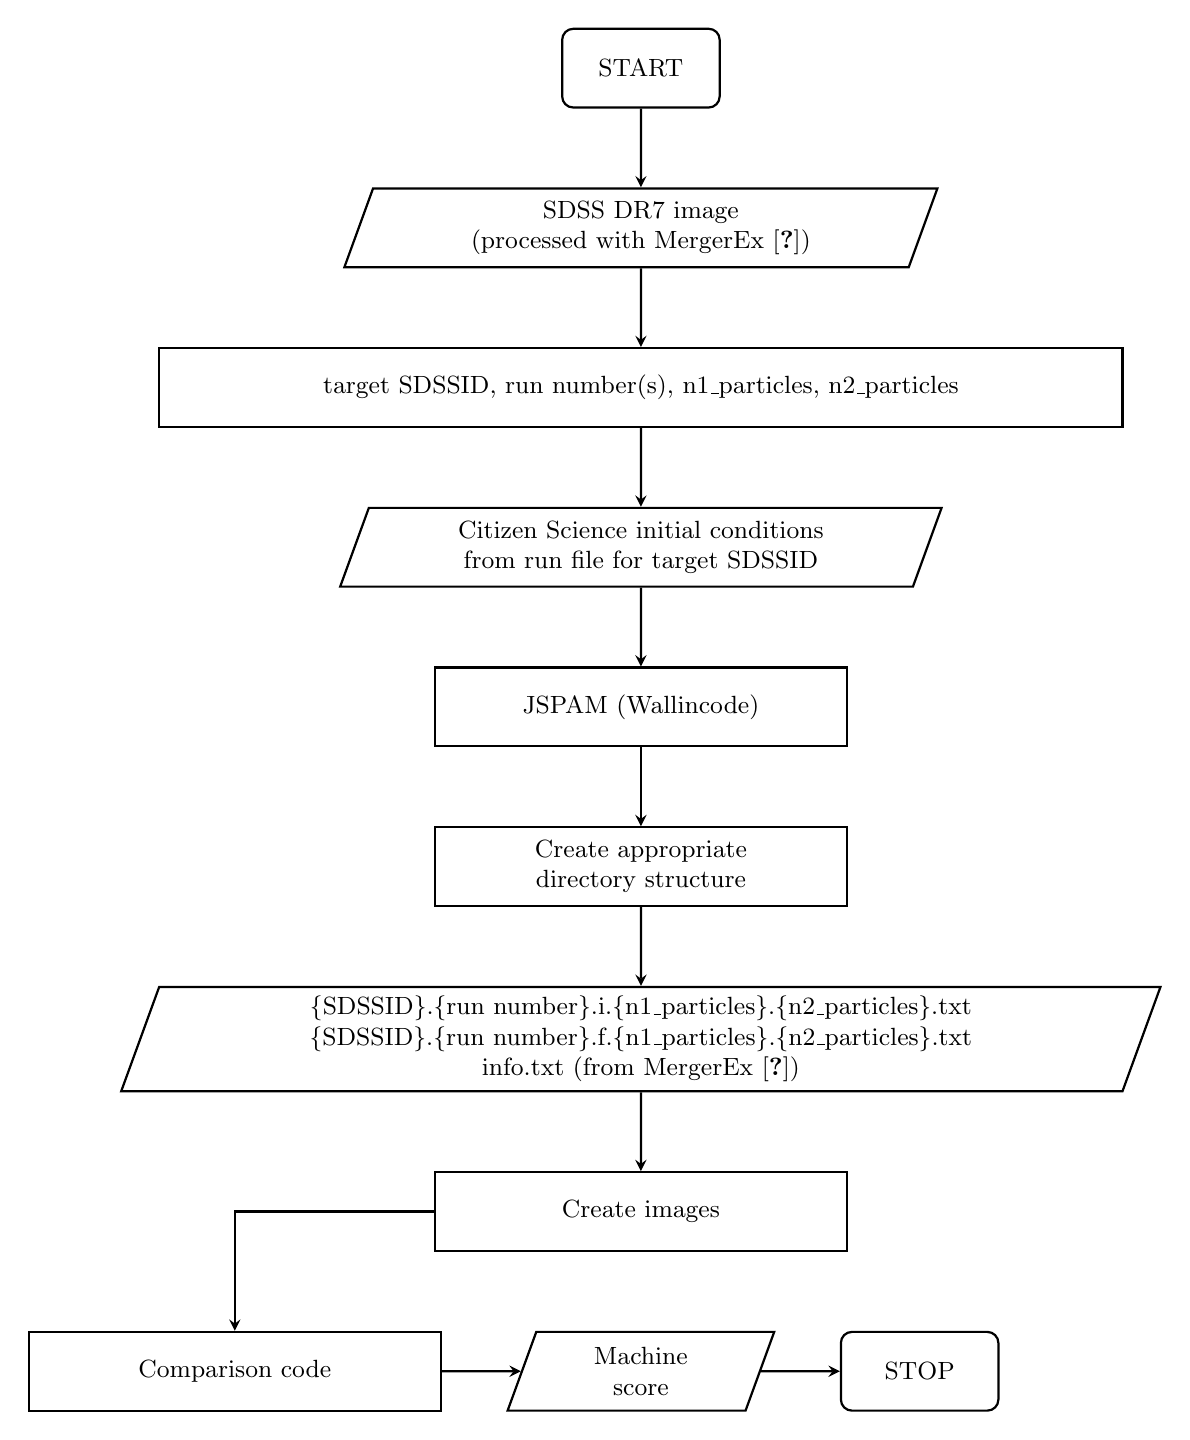
\begin{tikzpicture}[]
        \tikzstyle{every node}=[font=\small]
        \node [startstop] (start)
        {START};

        \node [io, below = of start, text width=6cm] (inData1)
        {SDSS DR7 image\\(processed with MergerEx \cite{holincheckThesis})};

        \node [process, below = of inData1, text width=12cm] (inData2)
        {target SDSSID, run number(s), n1\_particles, n2\_particles};

        \node [io, below = of inData2, text width=6cm] (inData3)
        {Citizen Science initial conditions\\from run file for target SDSSID};

        \node [process, below = of inData3] (JSPAM)
        {JSPAM (Wallincode)};


        \node [process, below = of JSPAM] (directories)
        {Create appropriate directory structure};

        \node [io, below = of directories, text width=12cm] (initialFile)
        {
        \{SDSSID\}.\{run number\}.i.\{n1\_particles\}.\{n2\_particles\}.txt\\
        \{SDSSID\}.\{run number\}.f.\{n1\_particles\}.\{n2\_particles\}.txt\\
        info.txt (from MergerEx \cite{holincheckThesis})
        };

        \node [process, below = of initialFile] (imageCreator)
        {Create images};


        \node [io, below = of imageCreator, text width = 2cm] (machineScore)
        {Machine score};

        \node [process, left = of machineScore] (comp)
        {Comparison code};

        \node [startstop, right = of machineScore] (stop)
        {STOP};

        \draw [arrow] (start) -- (inData1);
        \draw [arrow] (inData1) -- (inData2);
        \draw [arrow] (inData2) -- (inData3);
        \draw [arrow] (inData3) -- (JSPAM);
        \draw [arrow] (JSPAM) -- (directories);
        \draw [arrow] (directories) -- (initialFile);
        \draw [arrow] (initialFile) -- (imageCreator);
        \draw [arrow] (imageCreator) -| (comp);
        \draw [arrow] (comp) -- (machineScore);
        \draw [arrow] (machineScore) -- (stop);



    \end{tikzpicture}
    \caption[Project Flowchart]{
        Project flowchart. Here, it should be noted that our primary goal
        was developing a framework for testing comparison codes. This endeavor
        will likely see work in the near future.
    }
\end{figure}

\end{clearpage}

The primary motivation for having a machine scoring mechanism for these types of
simulations is to reserve human effort for distinguishing the best fitting
morphologies out of the good rendered morphologies. This is in contrast with the
current \textit{modus operandi}, which in some cases results in humans being
tasked with classifying a \textit{clearly} ill-fitting rendered morphology
as \say{bad}. If we can task a computer with making classifications that require
less acute discernment, humans in the
loop can be tasked with finding the \textit{best of the best} rendered
morphologies.

Therefore, we operate under the assumption that an ideal machine scoring
mechanism should be able to essentially recreate the results of the Galaxy Zoo:
Mergers Citizen Science effort nearly exactly.
However, in this work, we focus more on developing a framework to handle
running the simulation software efficiently, storing and organizing the large
volumes of data that are inherent to this project, accessing these data
efficiently, image creation, and image analysis.
In other words, while the ultimate goal for JSPAM is the creation of a general
purpose fitness function to compare the output of the JSPAM simulations to
the real systems it is supposed to model, the fitness function used in our
current working framework is largely a placeholder to ensure
that the framework is working properly score.
We recognize that further work must be done in developing fitness-functions, and
expect that our work will aid further success in doing so.

% ---------------------------------------------------------------------------- %
\subsection{Image Preparation and Target Data Acquisition}
% ---------------------------------------------------------------------------- %
The software we use for target image preparation and for constraining the
initial simulation parameter values is MergerEx, described in
\citet{holincheckThesis} and found at
\texttt{https://github.com/aholinch/MergerEx}. MergerEx greatly simplifies and
speeds up the process of querying various astronomical image servers for
specific sky coordinates, calibrating the images, and estimating initial
parameters that describe the sizes, orientations, and velocities of the
primary and secondary galactic disks in the merger.

Because the data in which we are interested is only the morphology, we can rely
on whichever images display the morphological features most clearly.
The MergerEx software allows us to choose the most appropriate image source from
either the NASA/IPAC Extragalactic Database/STScI Digital Sky Survey (NED/DSS),
or Sloan Digital Sky Survey Data Release 7, 8, or 9 (SDSS DR7, DR8, DR9).
For our purposes, neither the wavelengths comprising the images retrieved nor
the source matter as long as the distribution of luminous stars in the system is
shown in the image \cite{Holincheck2015}. In some cases, \citet{Holincheck2015}
describes that these images can even come from non-scientific data sets as long
as the previously mentioned condition is met.

\citet{Holincheck2015} provides a list of 54 SDSS and 8 Hubble Space Telescope
(HST) targets. For each of these targets, we follow the process for estimation
of the disks as described in Appendix C of \citet{holincheckThesis}.

Rather than leave this task up to users in future work,
a directory containing target images, the initial simulation parameters,
and the full-color press release images has been included in the project
repository, referenced in \ref{sec: appendix}.
% ---------------------------------------------------------------------------- %

% ---------------------------------------------------------------------------- %
\subsection{Input Storage: Targets and Target Input Files}
% ---------------------------------------------------------------------------- %
In many cases during this project, we wanted to work with \textit{only}
parameters that result in simulations that would have received a
Citizen Science score, and therefore elected to simply remove a significant
number of simulation parameters that resulted in a rejected simulation.

The input data files that contain the initial simulation
parameters are located in the \texttt{input} directory in the root directory
(\texttt{jspamcli.py} expects this to be their location).
These have been reduced in size from the
original files found at \texttt{https://data.galaxyzoo.org/mergers.html}, as
they now contain initial simulation parameters from scored runs. They are made
available in the GitHub repository.
% ---------------------------------------------------------------------------- %


% ---------------------------------------------------------------------------- %
%\subsection{JSPAM, Restricted three-body Simulations}\label{ssec: jspam}
% ---------------------------------------------------------------------------- %
%\todo[inline]{I was not able to add any review of restricted three-body
%    simulations as of yet. I will be adding more information here, as they are
%    essential for cutting down on computational time when the parameter space
%    is still too wide for any regular, beneficial, simulation of
%non-gravitational physics in full $n$-body simulations.}

%\todo[inline]{For some reason, I did not think to add a description of how the
%    actual simulation is run, as we did not write the simulation. Readers would
%    benefit from having this information included. I will be adding this in the
%future.}
% ---------------------------------------------------------------------------- %
% ---------------------------------------------------------------------------- %
\subsection{\texttt{merger} Python Package}
% ---------------------------------------------------------------------------- %
One of the primary challenges present in many projects in astronomy or
astrophysics is simply doing adequate book-keeping of data and related
information. This project is no different.
It was immediately necessary to develop a small,
purpose-built Python package to do just that. Within the \texttt{merger} package
found in the project repository, we make available the \texttt{MergerRun} and
\texttt{Galaxy} classes,
both of which are made available from the top level in the package. They can be
imported from the directory containing the merger package via
\say{\texttt{from merger import MergerRun, Galaxy}} or simply
\say{\texttt{from merger import .}}, although this second import statement also
imports a \texttt{data\_tools} package and \texttt{get\_target\_data} module which
will be described later.

Instantiation of a \texttt{MergerRun} is intended to require the fewest number
of arguments possible to reduce book-keeping. It does so by utilizing an
information file written by MergerEx during image preparation, which contains
a list of pertinent information. One of the member functions within the
\texttt{MergerRun} class simply turns this text file into a dict, which it then
initializes as several of the class instance attributes. An instance of this
class also requires the number of particles to be initialized in each disk, the
run number, and the initial simulation parameters that are found in the input
files. This can all be done in a statement such as

\begin{lstlisting}
merger_instance = MergerRun(path_to_info_file, n1_particles, n2_particles, run_number, init_sim_param_string)
\end{lstlisting}

Having a dedicated MergerRun class allows for \textit{all} of the necessary
information for a particular run of a merger to be passed between functions and
programs. While this method has potential to be a bit slower, we expect
programming using this class to remain a bit simpler and perhaps more clear.

This class also instantiates twice the \texttt{Galaxy} class,
one referred to as \texttt{primary} and the other referred to as
\texttt{secondary}. We can therefore more clearly keep track of the SDSS ID or
name, and regarding the disk centers, the right ascension and declination, and
the Cartesian coordinates relative to the pixels in the frame.

Within this package also a small package called \texttt{data\_tools} containing,
as of writing, one class called \texttt{Structure}. \texttt{Structure} accepts
an ordered list of directory and subdirectory names that will comprise a
directory structure to be created. In other words, the following code block

\begin{lstlisting}
dir_structure = Structure(["root_name", "child_1", "child_2", "child_3"])
\end{lstlisting}

will create the following path in your current working directory:
\texttt{root\_name/child\_1/child\_2/child\_3/}. Although this may seem
unneccessary, this reduces the chance of error in organization of the large
volume of simulation data that will be produced.

Further, in the top level of the package also exists \texttt{get\_target\_data}.
This is a module that specifically scrapes
\texttt{https://data.galaxyzoo.org/mergers.html} for all of the
available target data, allows for a user to select from the targets available,
downloads and unarchives the data into an \texttt{input} directory in the
working directory. This is more apparently useful in the interactive
mode of \texttt{jspamcli.py}.
% ---------------------------------------------------------------------------- %

% ---------------------------------------------------------------------------- %
\subsection{JSPAM Command Line Interface (\texttt{jspamcli.py})}
% ---------------------------------------------------------------------------- %
The original JSPAM code described in \citet{Wallin2016} can be called from
the command line via \texttt{./basic\_run} with a required string argument of
initial simulation parameters, and it accepts a number of options to specify
run settings and simulation quantities such as the number of particles to
be initialized around each center, for instance. While essentially all the
existing functionality has been fundamentally unchanged, we set out to make
interaction with the software more user friendly and intuitive.
Further, we wanted to
initiate the minimization of the human-in-the-loop even in the initial program
setup for new users.
After the Fortran90 code is compiled, users can run \texttt{jspamcli.py} using
Python3. This program can be run in four modes selected via command line
options. These modes are given as follows:
\begin{table}[h!]
    \centering
    \begin{tabular}{clll}
    \toprule
    Mode & Option       & Behavior                        & Arguments \\
    \midrule
    $1$ & \texttt{-i}  & run interactively               & NONE          \\
    $2$ & \texttt{-bi} & batch process interactively     & NONE          \\
    $3$ & \texttt{-b}  & batch process (normal)%
        & \texttt{batch\_run\_file}\ldots\\
    $4$ & \texttt{-bm} & batch process on multiple cores & \texttt{num\_cores}
    \texttt{batch\_run\_file}\ldots\\
    $5$ & \texttt{-g}  & GIF Creation Tool              & NONE          \\
    \bottomrule
    \end{tabular}
    \caption[\texttt{jspamcli.py} command line options]{List of command line options
        available in \texttt{jspamcli.py}. In the \texttt{-b} and \texttt{-bm}
    modes, multiple batch run files may be specified as long as they exist in
    the \texttt{batch\_run\_files} directory in the root directory.}
\end{table}
Mode $1$ allows interactive processing of multiple runs of one
target and can be called by \texttt{python3 jspamcli.py -i}.
Interaction with JSPAM is easy in this context, as all options are
handled interactively. The user is given an option to download input files using
the \texttt{get\_target\_data} module, and then can choose from available input
files to run the program. The user is then asked to enter the number of
particles to be initialized in each galaxy. Then, the program runs in
essentially the same way as in the batch processing modes.

Before \texttt{jspamcli.py} can be run in any of the batch processing modes
(modes $2-4$), one or more batch run files must be specified. If none are
specified, the program writes out a sample batch run file named
\texttt{sample.txt} in the \texttt{batch\_run\_file} directory.
The contents are below:
\begin{verbatim}
#target,n1_particles,n2_particles,first_run,last_run
587722984435351614,500,500,100,100
\end{verbatim}
However, if in the last column of a row there is the keyword \texttt{ALL}, the
values given for \texttt{first\_run} and \texttt{last\_run} are ignored
and all available non-rejected scored runs are processed. This file would read
\begin{verbatim}
#target,n1_particles,n2_particles,first_run,last_run
587722984435351614,500,500,000,000,ALL
\end{verbatim}

Modes $2-4$ are variations on batch processing modes and all make
use of the available batch run files.
Mode $2$ essentially gives the user an
introduction to how batch processing is handled by \texttt{jspamcli.py} and is
useful in contexts where the job to process does not have to be left running
for a exceedingly long duration of time.

Mode $3$ has all of the functionality of mode $2$ but none of the interactivity.
This mode runs as one would expect and processes all desired runs sequentially.

Mode $4$ contains methods for parallelizing the \texttt{basic\_run} process.
We wanted to minimize the need to change the original Fortran90 code, so the
Python \texttt{multiprocessing} module was used parallelize the execution of
the JSPAM simulation via \texttt{basic\_run} across multiple processors with
different arguments passed to the simulation in each.
While this does not necessarily reduce the time needed for any one simulation,
as JSPAM has not necessarily been parallelized itself,
this does reduce the amount of time
required to run a large number of simulations fairly quickly just by simply
doing more things at the same time. We can fairly easily significantly
speed up our workflow by making use of the cores available to us on any
workstation or machine.

Within the \texttt{multiprocessing} module is a \texttt{Pool} object that
accepts an argument indicating the number of worker processes to be spawned.
Upon execution of \texttt{jspamcli.py}, the argument passed to the program
indicating the requested number of cores to be used is used to instantiate the
\texttt{Pool} object (although we limit the number of cores to be used to half
of those available to preserve resources and good relations with other users).
Each execution of \texttt{basic\_run} using a
particular set of simulation parameters is considered to be completely
independent of all other processes, as the inputs for each simulation do not
depend on the results of the previous simulations. Therefore, we care very
little if all simulations requested run sequentially. We can therefore use the
\texttt{map\_async} module to distribute calls to the appropriate calling
function across the spawned worker processes.

Although we can now execute \texttt{basic\_run} processes across multiple cores,
we needed to take into account that this program writes out the initial and
final simulation data file. While the processes are not using a shared memory
location during the run, they are writing out these files to the same location.
The simple fix was to add an \texttt{-m} flag in \texttt{basic\_run} that
indicates that the program should insert a distinguishing number corresponding
to the process number in the name of the file. This allows for
\texttt{jspamcli.py} to organize the output files appropriately.
% ---------------------------------------------------------------------------- %


% ---------------------------------------------------------------------------- %
\subsection{Output Storage: Directory and File Naming Conventions}
% ---------------------------------------------------------------------------- %
We explored the possibility of adopting binary data
formats such as HDF5 rather than defaulting to flat files to store data.
While making use of binary data formats either by implementing an
IO interface that works across our existing programs in Fortran90, Python,
and C++ or by simply using HDF5 could potentially reduce IO overhead, it was
determined to not be an effective use of time at this point in the project.
Therefore, flat ASCII files are the working paradigm until another
solution is deemed necessary.

Because we are using flat files, we adopted a standard naming convention for all
output files regardless of their storage location. For any one particular run of
the JSPAM code, we identify a unique output file via the SDSSID or name used,
the run number corresponding to the line number in the input file, a flag
indicating whether the data corresponds to the initial output or the final
output, and the number of particles initialized in each galaxy. The output files
for a unique run would have the form

\begin{verbatim}
name.run_number.i.n1_particles.n2_particles.txt
name.run_number.f.n1_particles.n2_particles.txt
\end{verbatim}

Further, we needed to have an appropriate directory tree set up for any
particular run. We can visualize this tree in figure \ref{fig: the_tree}
\begin{figure}[h!]
    \dirtree{%
        .1 root.
        .2 output.
        .3 \{SDSSID\}.
        .4 \{SDSSID\}.humanscores.txt.
        .4 run0000.
        .5 \{SDSSID\}.0000.i.\{n1\_particles\}.\{n2\_particles\}.txt.
        .5 \{SDSSID\}.0000.f.\{n1\_particles\}.\{n2\_particles\}.txt.
        .4 run0001.
        .5 \{SDSSID\}.0001.i.\{n1\_particles\}.\{n2\_particles\}.txt.
        .5 \{SDSSID\}.0001.f.\{n1\_particles\}.\{n2\_particles\}.txt.
        .4 run0002.
        .5 \{SDSSID\}.0002.i.\{n1\_particles\}.\{n2\_particles\}.txt.
        .5 \{SDSSID\}.0002.f.\{n1\_particles\}.\{n2\_particles\}.txt.
        .4 run\ldots.
        .5 \{SDSSID\}.\{\ldots\}.i.\{n1\_particles\}.\{n2\_particles\}.txt.
        .5 \{SDSSID\}.\{\ldots\}.f.\{n1\_particles\}.\{n2\_particles\}.txt.
    }
    \caption[Output directory tree]{Output directory tree}
    \label{fig: the_tree}
\end{figure}


At this point \texttt{jspamcli.py} only needs minor additions to work with
the rendered image creation software and difference code which comprised the
other half of this project. Incorporating all pieces of the project in an
automated machine learning framework would require only a few augmentations,
to the existing code, and would support the ultimate goal of optimizing
the parameter space for better convergence on solutions.
This is likely to be explored in continuing research on this project.

% ---------------------------------------------------------------------------- %
% COMMENTED OUT
% ---------------------------------------------------------------------------- %
\begin{comment}
\subsection{Fitness-function Development}\label{ssec: fitness}
The primary goal of this work as a whole is to make progress on the
development of a fitness-function that will return some kind of machine score.
If we find an efficient method for determining convergence of models on the
observed morphologies that rivals that of a human fitness-function, we can then
begin using this method for real-time analysis of models. Although human
fitness-functions are robust and can make use of our innate pattern-matching
abilities \cite{Holincheck2015}, the ability to determine model convergence more
precisely with improved fitness-functions in
sequence with simulations immediately opens the door to improving the results
of previously applied genetic algorithms and applying new machine learning
techniques for optimizing the parameter space for all possible solutions.

That being said, we would be \textit{wrong} to not acknowledge the innate pattern-recognition abilities of humans that made the success of the Galaxy Zoo
project successful \cite{Holincheck2015}.
Rather than abandoning human interaction altogether once
a successful method for machine scoring is in place, perhaps a better approach
is to allow the machine scoring mechanism remove \say{bad} simulations from the
set that needs to receive a human score, effectively reducing the human choice
from the best of \textit{all} solutions to the best of \textit{good} solutions.

\todo[inline]{The current method of comparison is a simple normalization and
subtraction of translated images.}
\end{comment}
% ---------------------------------------------------------------------------- %
% COMMENTED OUT
% ---------------------------------------------------------------------------- %

% ---------------------------------------------------------------------------- %
%\subsection{Fitness-function Analysis}
% ---------------------------------------------------------------------------- %
%\todo[inline]{
%    This section currently has no information because no work has been done in
%    support of this section. Once we have several fitness functions working,
%    we will begin analyzing. I think since this is the primary goal of the
%    project, it really should live in the ANALYSIS section.
%}

%\subsection{Optimization of Initial Parameter Space}
%\todo[inline]{There will be more information added here in future when
%we arrive at this stage in the project, but I think that this will likely be
%better explored in continued research rather than the thesis.}




\section{Results}
The primary objective in carrying out this project was to build an
infrastructure to support the investigation into methods of
optimization of initial simulation parameters based on the output of the
JSPAM simulations.
We have accomplished this objective by establishing a working framework with a
elementary approach at comparison of simulation images and real SDSS DR7, DR8,
and DR9 images prepared with MergerEx.

There now exists a dedicated
\texttt{merger} class with member functions that implement most necessary tasks
relating to the merger data. Rather than deal with data I/O on a case by case
basis, we can now instantiate this class to encapsulate all necessary data for
operations common to analysis of mergers in the context with which we are
concerned. Further, the output from all member functions has been logically
structured to reduce future headaches that come from handling large volumes
of file I/O. There also exist several member functions that aid in visualization
of a particular simulation from start to finish.

The \texttt{merger} class is used extensively in what we dub the JSPAM Command
Line Interface (\texttt{jspamcli.py}). This program makes interacting with
the JSPAM code a bit more intuitive and gives the user several modes of
interaction that we found to be useful in different contexts. Further, we have
now standardized I/O from JSPAM so that future work on the project can rely on
predictable I/O behavior.

We also created an option to execute \texttt{basic\_run} asynchronously across
a variable number of cores. While we have not strictly parallelized
\texttt{basic\_run}, we've distributed its execution to make more efficient use
of powerful workstations that are readily available.


\section{Analysis}
\textcolor{red}{At this point, there are no results to analyze as the project
is still in development.}


\section{Conclusions}
While our goal of establishing an interface for using and
interacting with data from the JSPAM code has been achieved,
it is clear that this work really lies mostly in a support role of other
projects. That being said, successful data-intensive projects rely heavily on
user-friendly data pipelines that handle most of the tedious labor and keep
track of all relevant data in a predictable, well thought-out manner.
We expect that the framework
we have created will be useful in that it lessens the overhead necessary to
bootstrap a project using the JSPAM code for its simulation software by
eliminating the need to create ad-hoc methods for interacting with the
simulation data. At this point, users are instructed on how to best interact
with the software for their needs using \texttt{jspamcli.py}, and there is a
clear method by which the simulation output data is stored and organized.

Because this framework is now well established, it becomes trivial to set
up a batch
run file to produce \textit{all} 66,395 sets of run data and then the
associated rendered images.
Essentially, this gives us a massive set of ranked simulation data that
can serve as a training set for future attempts at improving the results of
JSPAM by applying machine learning techniques.

We recognize near the time of completion of this phase of the project that it
would be quite useful to have a JSPAM interface object that can be used
programmatically and that accepts an initial run string as an argument to a
\say{run} method. In tasks where these initial condition guesses are being
optimized, having an implementation of this would be essential for rapid
testing.

While this project has not arrived at scientific results, we intend for our
code to handle some of the
heavy lifting in future projects electing to use the JSPAM code.

% --------------------------------------------------------------------------- %

% --------------------------------------------------------------------------- %
% Bibliography
% --------------------------------------------------------------------------- %
\clearpage
\bibliography{thesisbib}
% --------------------------------------------------------------------------- %

\end{document}
